\documentclass[addpoints,11pt,a4paper]{exam}
\usepackage[margin=1in]{geometry}
\usepackage{amsmath, amsfonts}
\usepackage{pythonhighlight}
\usepackage{graphicx} %package to manage images
% \usepackage{exam}
\usepackage{pgfplots}

\graphicspath{ {./images/} }
\printanswers
\begin{document}
\begin{center}
{\Large {\textbf{Spring 2024}}}\vspace{1.0em}\\
{\Large {\textbf{CS 412 (Algorithms: Design and Analysis)}}}\vspace{1.0em}\\
{\Large {\textbf{Weekly Challenge 01: Getting Started...}}}\vspace{1.0em}\\
{\Large {Announced: Friday, January 12, 2024. Deadline: Friday, January 19, 2024 (11:59 pm PST). Total marks: \numpoints.}}\vspace{.5em}\\
\end{center}
Instructions: Submit *individually* your solution as PDF with the file name as your studentID.pdf; typset in LaTeX. You must submit your solution on Canvas.

\centerline{\rule{.7\textwidth}{1pt}}

\begin{questions}
\question[1]
\
{\textbf{Formal definition of Big-Oh:} Welcome to CS 412! For the first weekly challenge, recall the formal definition of Big-Oh as:

$f(n)$ is $O(g(n))$ if there exist positive numbers $c$ and $n_0$ such that 
		$f(n) \leq c g(n)$, for all $n \geq n_0$.
}

Let's try to find the constants $c$ and $n_0$ for the time complexity of some algorithm characterized by a function $f(n) = 2n^2 + 3n + 1 = O(n^2)$ 

We can find these constants algebraically but let's plot the running time of $c g(n)$ for different values of $c$ and $n_0$. You may use the values for $N$ ($n_0$) starting with 1, 2, 3, 4, and 5 (see the table below).

Plot the function $f(n)$ together with $g(n)$ [with different values of $c$ and $n_0$; with values of $n_0$ on the $X-axis$ and the corresponding values of $f(n)$ and $c g(n)$ on the $Y-axis$. 

What is the smallest value of $c$ and $n_0$ where $f(n) = O(g(n))$? Briefly comment [in two to three sentences only] on any notable observations drawn from this little exercise. 
\includegraphics[width=1.0\linewidth]{image.png}
\begin{solution}
    The graph illustrates that the convergence of different values of the constant "c" is essential for the equation to adhere to the Big-O notation (O(g(n))). The visual representation indicates that values of "c" greater than 2 facilitate the convergence of the graph at some point, ensuring that f(n) closely aligns with the upper bound O(g(n)). The graphical analysis along with algebraic verification highlights that for c = 6, the corresponding minimum N value is 1, establishing it as the N0 for the function
    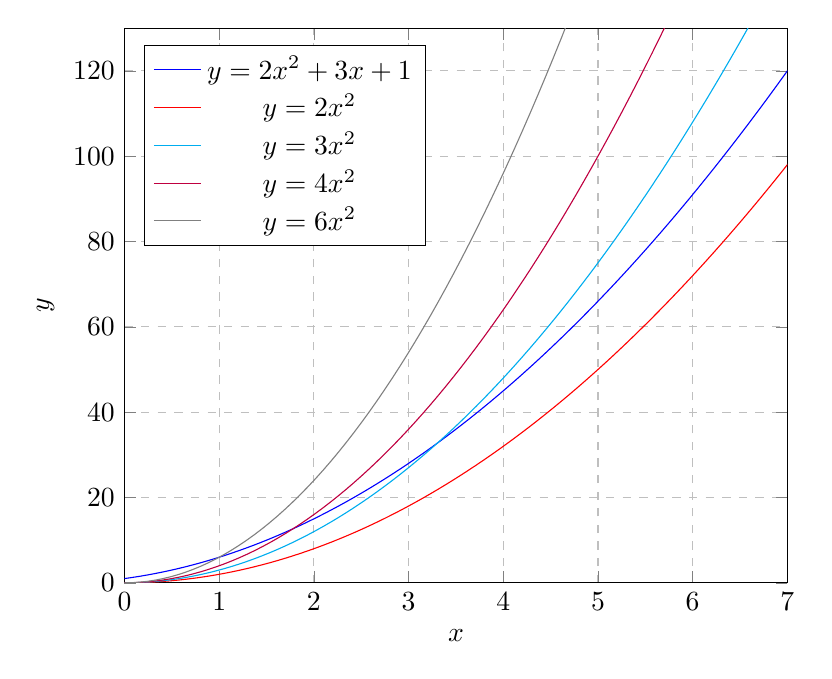
\begin{tikzpicture}
        \begin{axis}[
          xlabel={$x$},
          width=10cm,
          ylabel={$y$},
          xmin=0, xmax = 7,
          ymin=0, ymax = 130,
          legend pos = north west,
          grid=both,
          grid style = {dashed},
        ]

        \addplot[blue, domain=0:8, samples=100] {2*x^2 + 3*x + 1};
        \addlegendentry{$y = 2x^2 + 3x + 1$}
        
        \addplot[red, domain=0:8, samples=100] {2*x^2};
        \addlegendentry{$y = 2x^2$}
        
        \addplot[cyan, domain=0:8, samples=100] {3*x^2};
        \addlegendentry{$y = 3x^2$}
        
        \addplot[purple, domain=0:8, samples=100] {4*x^2};
        \addlegendentry{$y = 4x^2$}
    
        \addplot[gray, domain=0:8, samples=100] {6*x^2};
        \addlegendentry{$y = 6x^2$}
    
        % \addplot[black, domain=0:10, samples=100] {2*x^2};
        % \addlegendentry{$y = 2x^2$}
        %   % Quadratic equation 1: y = x^2
        %   \addplot[blue,domain=-2:2, samples=100] {x^2};
        %   \addlegendentry{$y = x^2$}
      
        %   % Quadratic equation 2: y = -x^2 + 4
        %   \addplot[red,domain=-2:2, samples=100] {-(x^2) + 4};
        %   \addlegendentry{$y = -x^2 + 4$}
      
        %   % Quadratic equation 3: y = 0.5x^2 + 2
        %   \addplot[green,domain=-2:2, samples=100] {0.5*x^2 + 2};
        %   \addlegendentry{$y = 0.5x^2 + 2$}
      
        \end{axis}
      \end{tikzpicture}
\end{solution}

\question[1] In computer science, $lg (n)$ by default refers to $log$ to the base $2$. The log function appears frequently in algorithm analysis and often, we ignore the base when performing asymptotic analysis. Does base really matter in asymptotic analysis? Plot the function $lg (n)$ with bases $2, 7, 10, 100$ for 'large values' of $n$. Write your observations (in two to three sentences only).

\begin{solution}
    As observed in the plot below, increasing the bases scales the graph vertically while the shape and growth rate is same, thus base is ignored as asymptotic notation focuses on the growth rate of functions instead of their absolute value.
    
    \includegraphics[width=1.0\linewidth]{q2.png} % Replace 'example-image' with your image file name and extension
    
\end{solution}

\end{questions}
\end{document}
